\begin{frame}[t]{Performance Evaluation\only<2->{ - Throughput}}
  \vspace{0.15cm}

  \only<2->{
    \begin{itemize}
      \setlength\itemsep{0.15cm}
      \item Cyclic dataflow that repeatedly performs all-to-all data exchange of a fixed number of records.
      \item Ideal aggregate throughput based on Ethernet Bandwidth.
      \item .NET Socket demonstrates achievable throughput given network topology, TCP overheads and .NET API costs.
      \item Naiad throughput scales linearly.    
    \end{itemize}

    \vspace{0.15cm}
    \begin{center}
      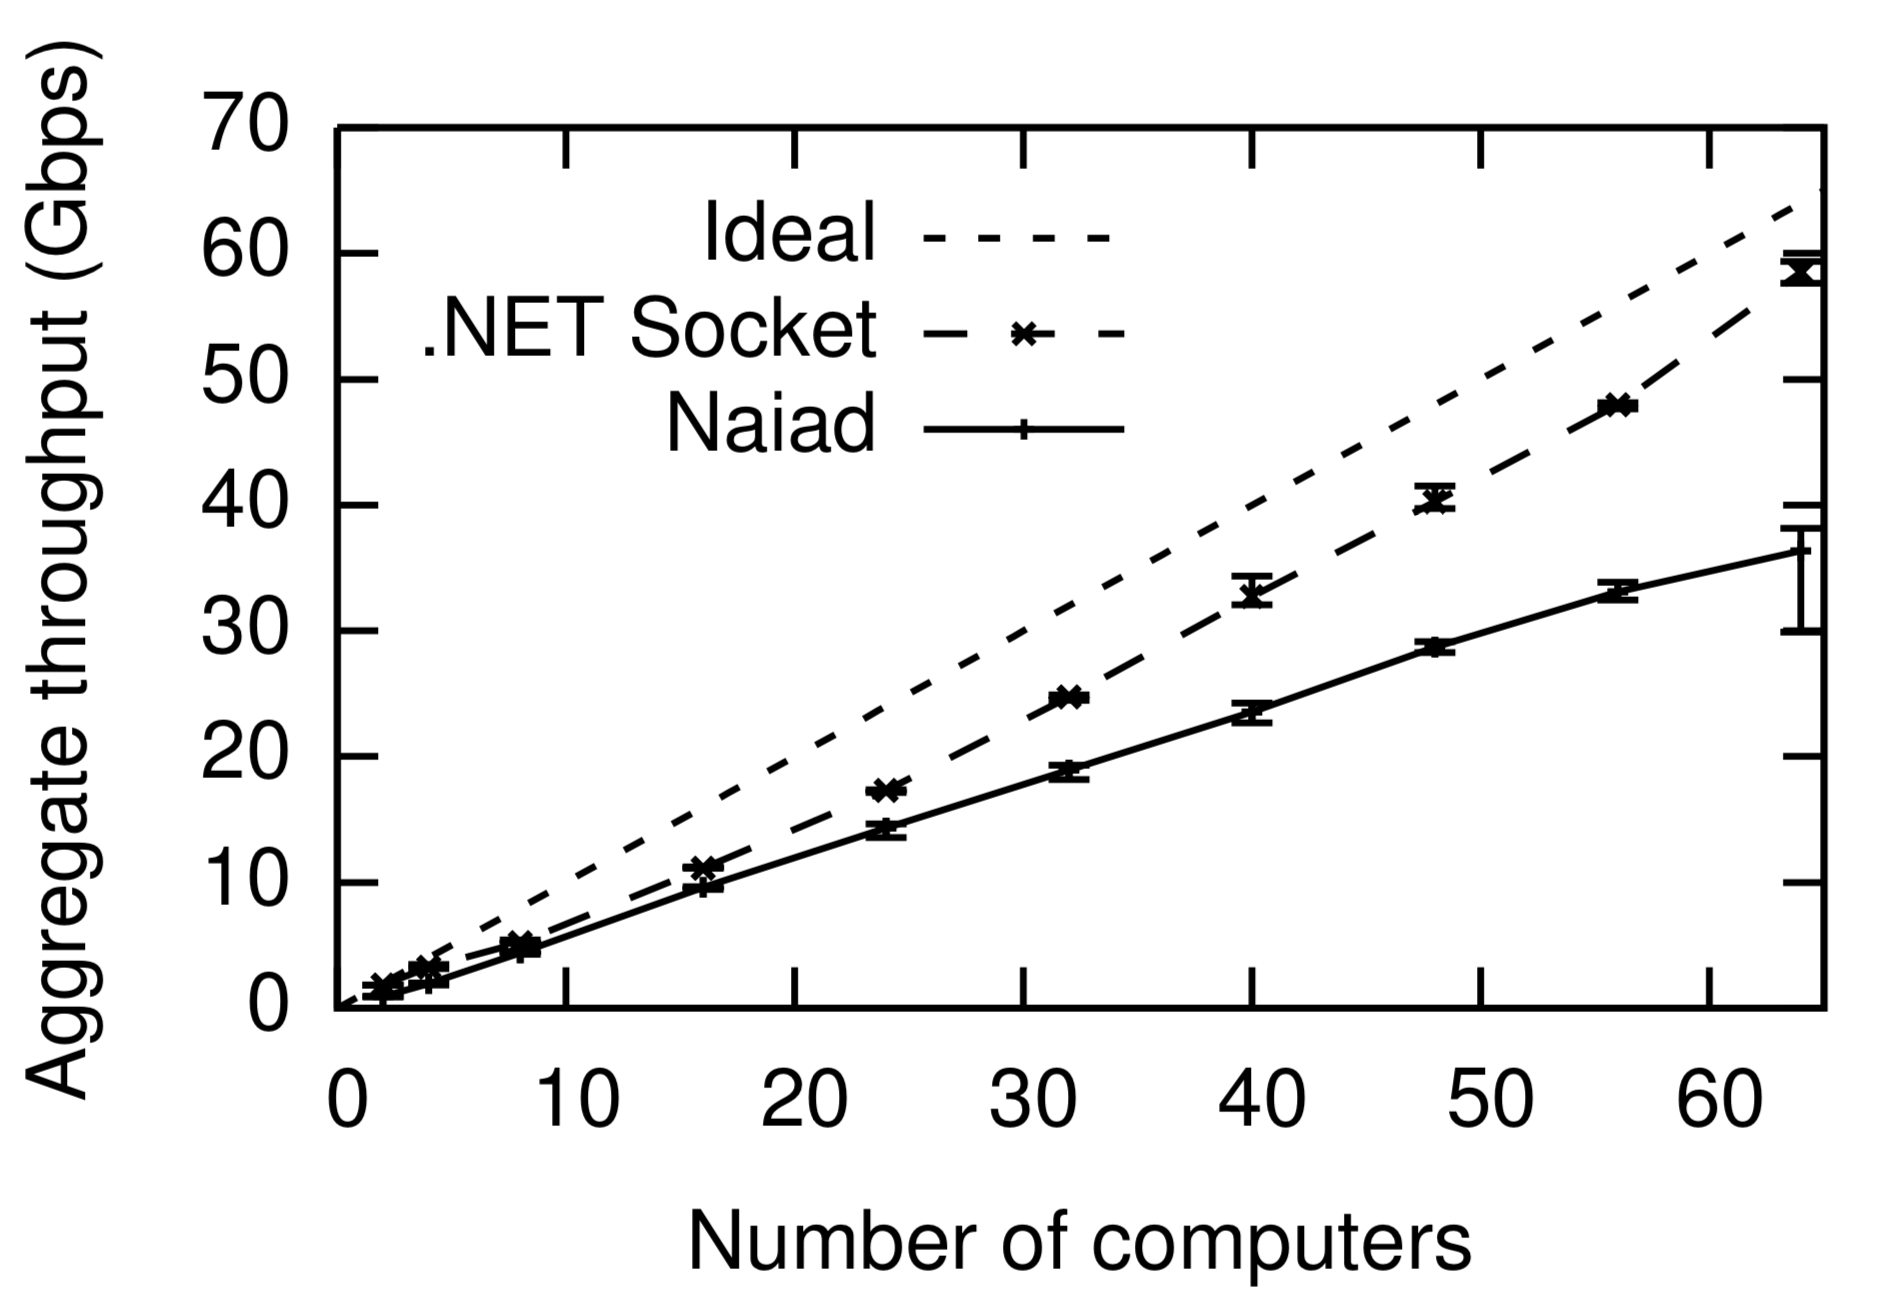
\includegraphics[width=0.55\textwidth]{6a}
    \end{center}
  }
\end{frame}

\begin{frame}[t]{Performance Evaluation - Latency}
  \vspace{0.15cm}

  \begin{itemize}
    \setlength\itemsep{0.15cm}
    \item Minimal time required for Global Coordination.
    \item Request and receive completeness notifications.
    \item Median time per iteration small at 753$\mu$s for 64 computers.
    \item 95th percentile results -– adverse impact of micro-stragglers.
  \end{itemize}

  \vspace{0.15cm}
  \begin{center}
    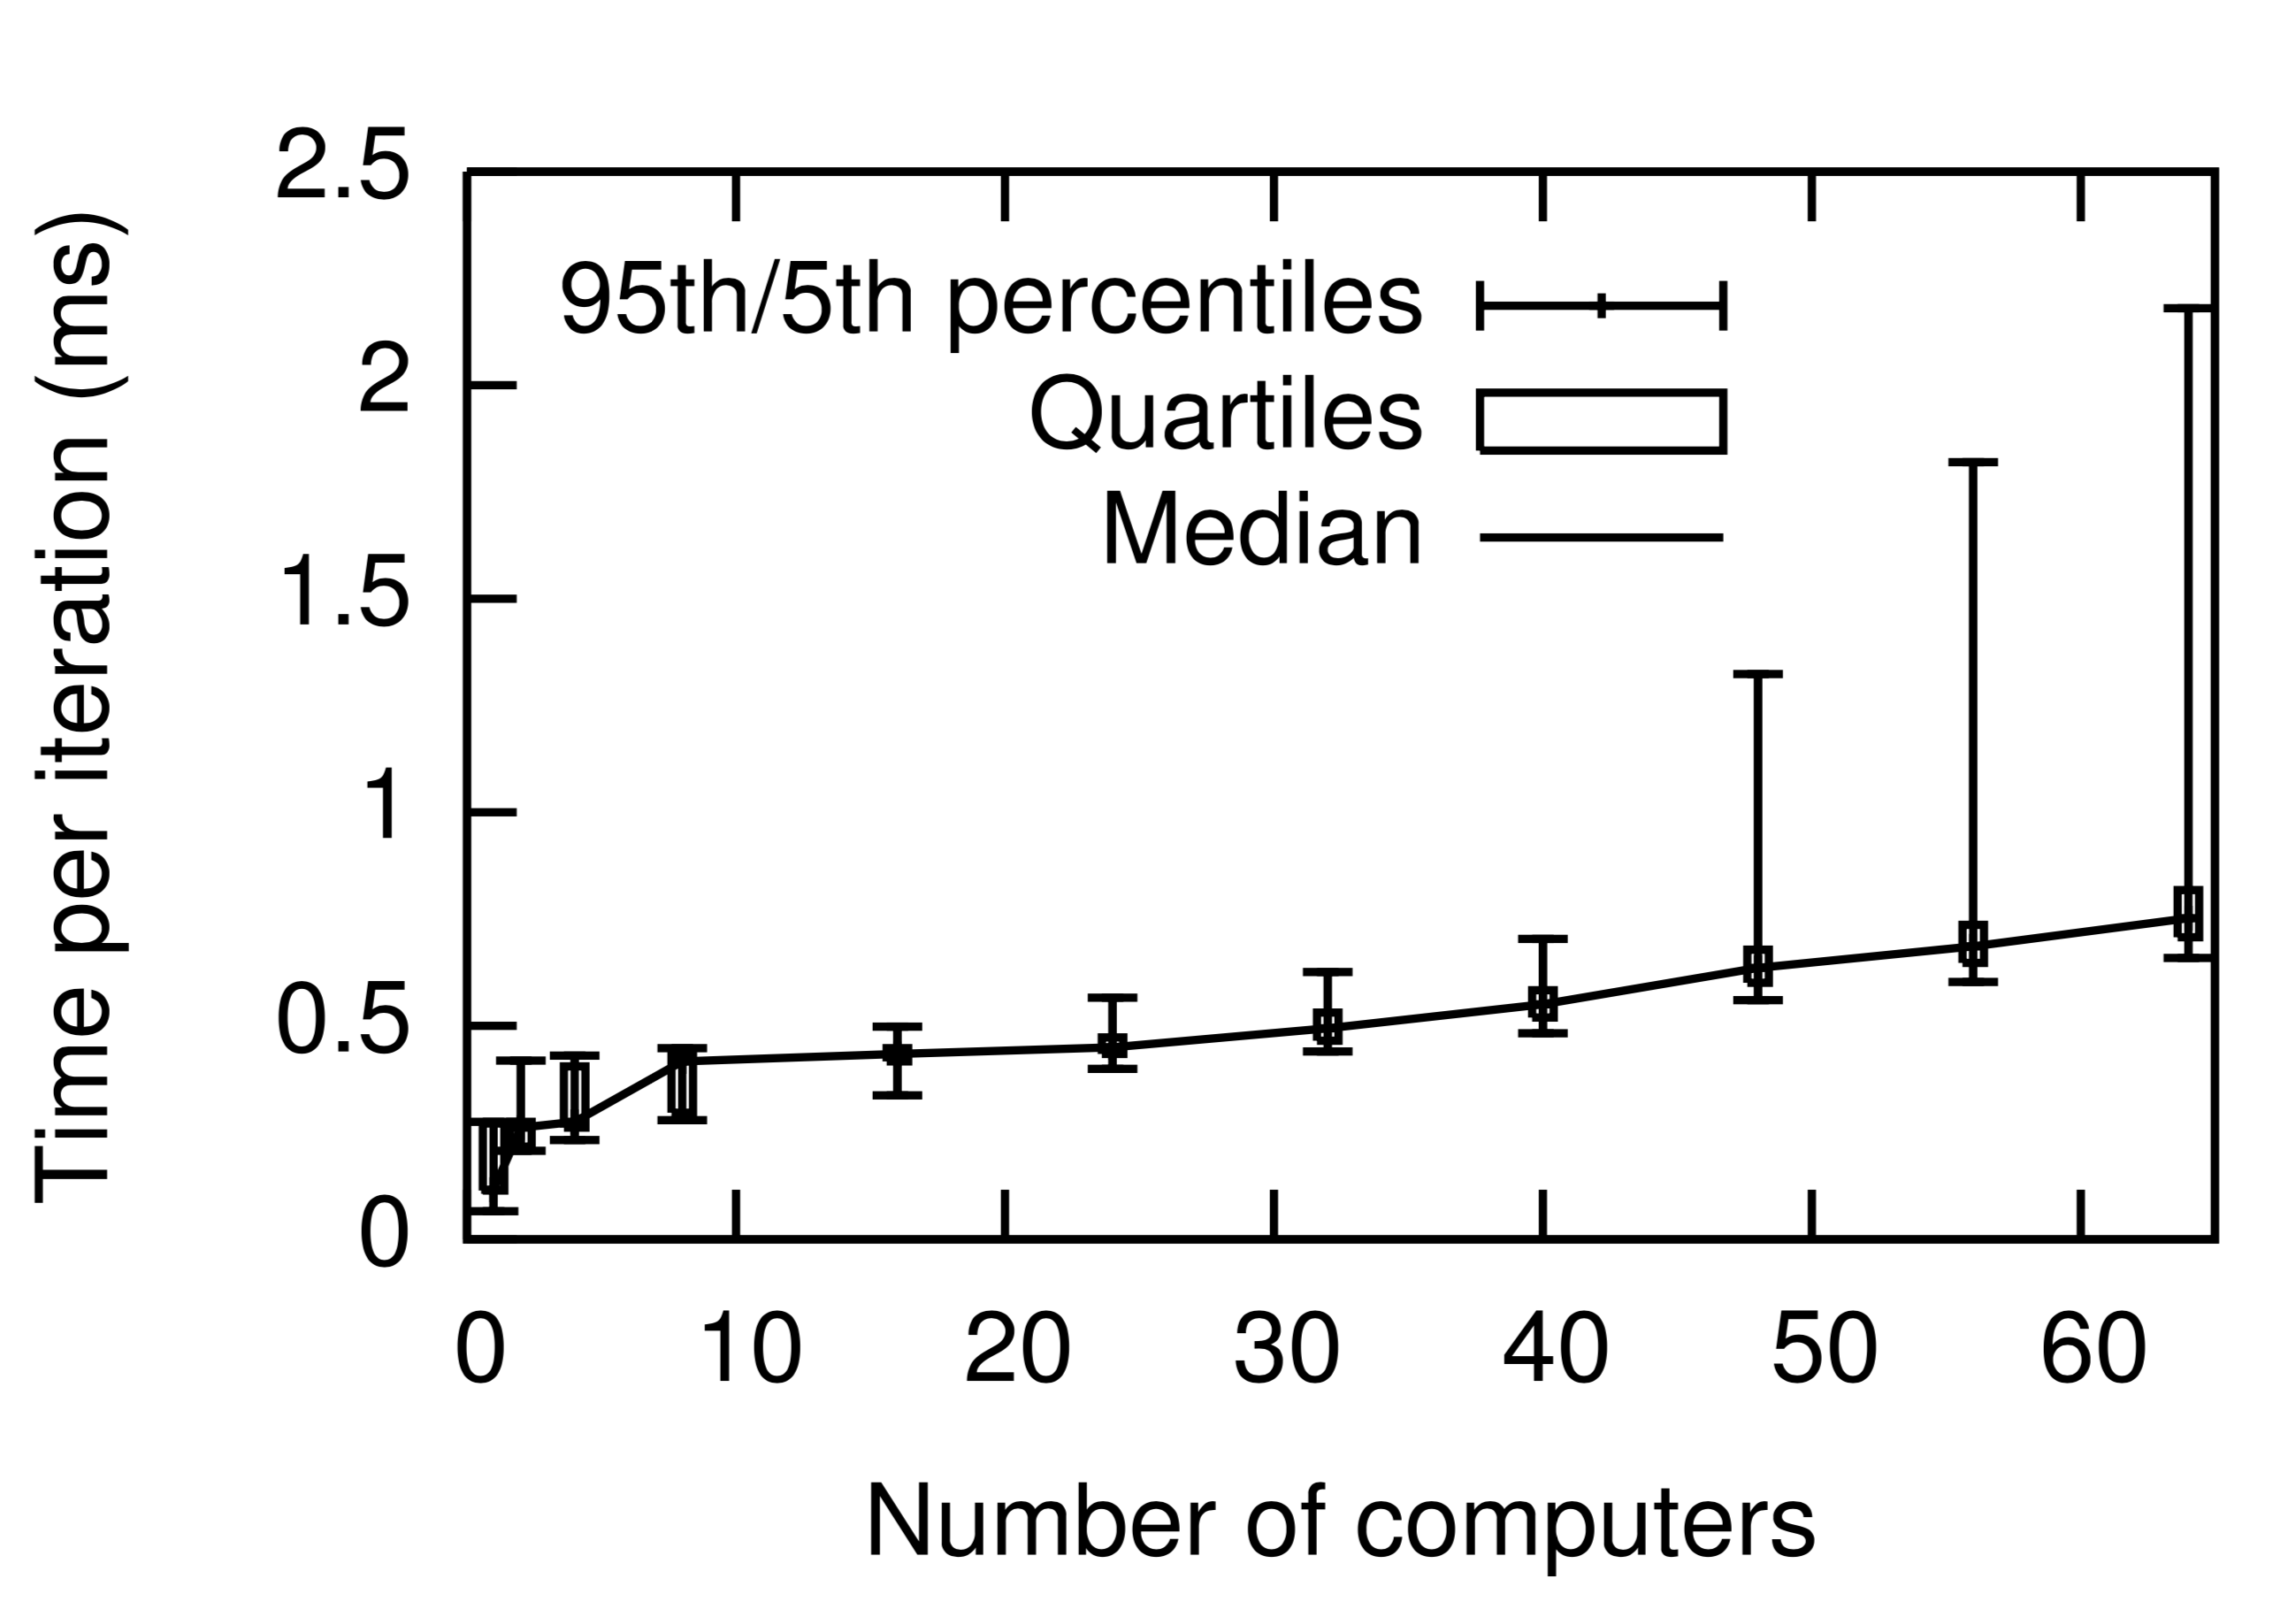
\includegraphics[width=0.55\textwidth]{6b}
  \end{center}
\end{frame}

\begin{frame}[t]{Performance Evaluation - Protocol Optimizations}
  \vspace{0.15cm}

  \begin{itemize}
    \setlength\itemsep{0.15cm}
    \item Weakly Connected Components Computation (WCC) on random graph of 300 edges (~2.2GB of raw input).
    \item Reduction in volume of protocol traffic depending on level of accumulation.
    \item In practice, reduction in messages from local accumulation is sufficient.
  \end{itemize}

  \vspace{0.15cm}
  \begin{center}
    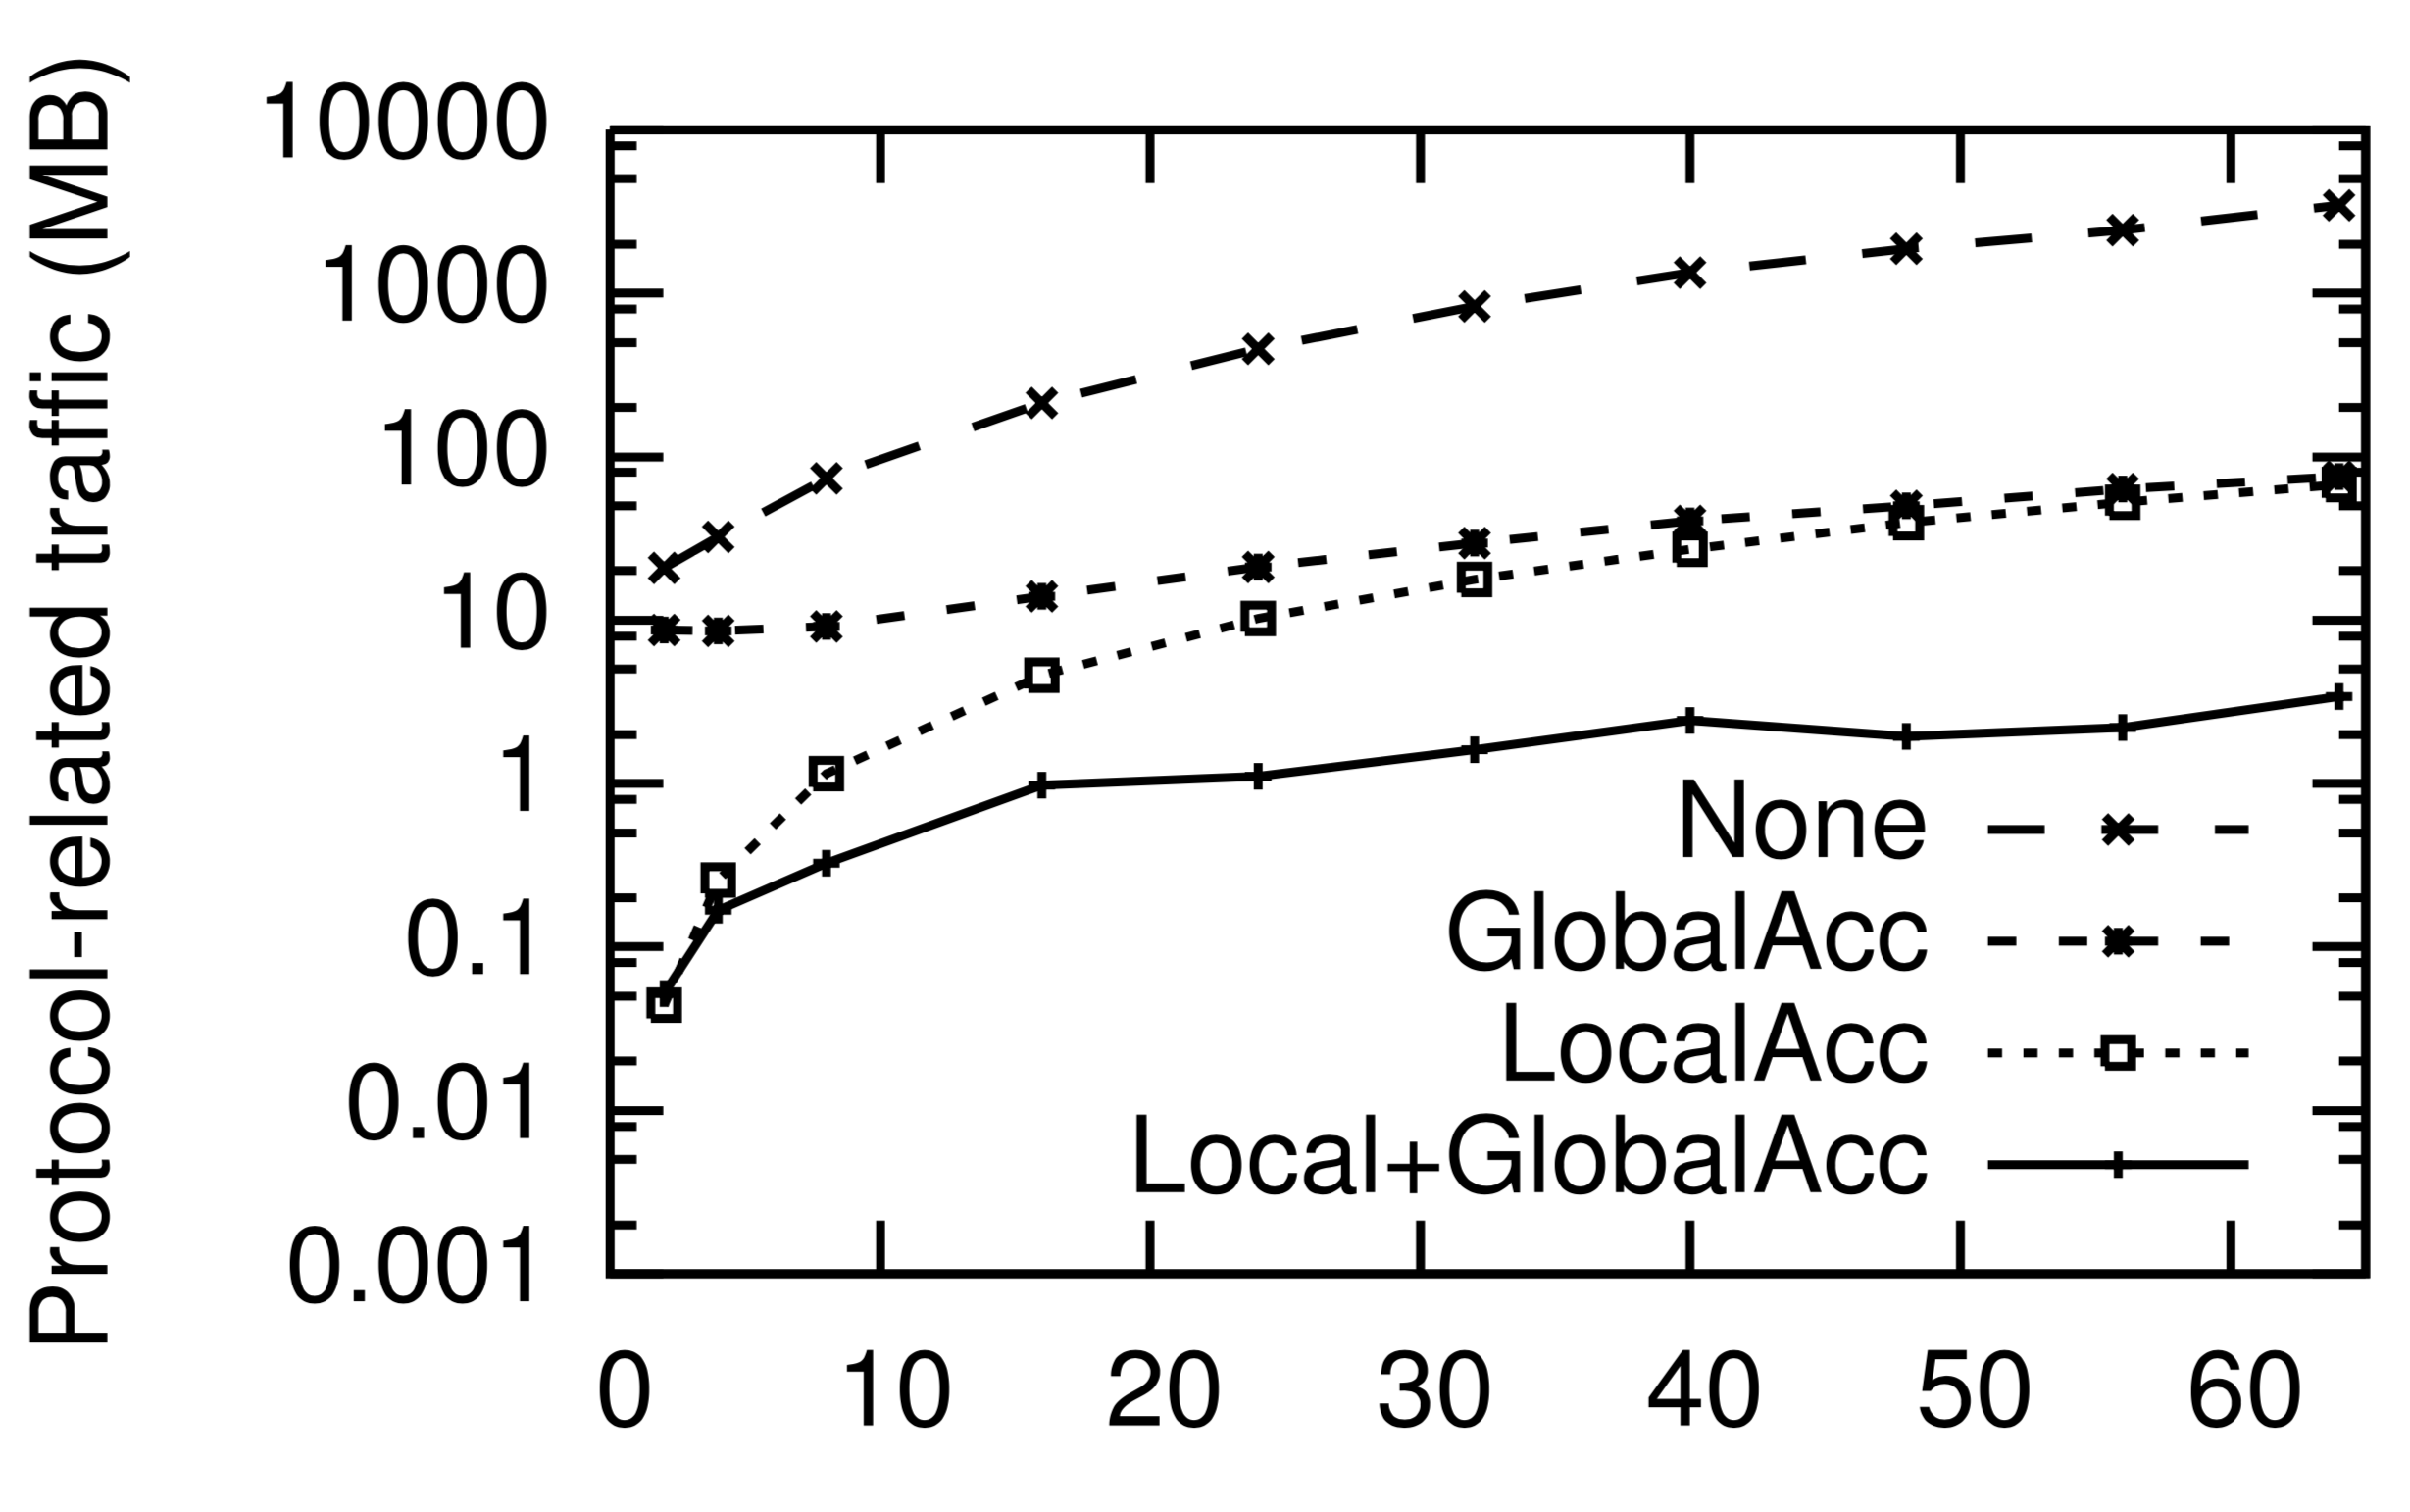
\includegraphics[width=0.55\textwidth]{6c}
  \end{center}
\end{frame}

\begin{frame}[t]{Performance Evaluation - Scaling}
  \vspace{0.15cm}

  \begin{itemize}
    \setlength\itemsep{0.15cm}
    \item Strong scaling – Adding compute resources with fix input size.
    \item Weak scaling – Adding compute resources and increasing input.
    \item Word Count – 128GB uncompressed corpus.
    \item WCC – Random Graph of 200M edges.    
  \end{itemize}

  \vspace{0.15cm}
  \begin{center}
    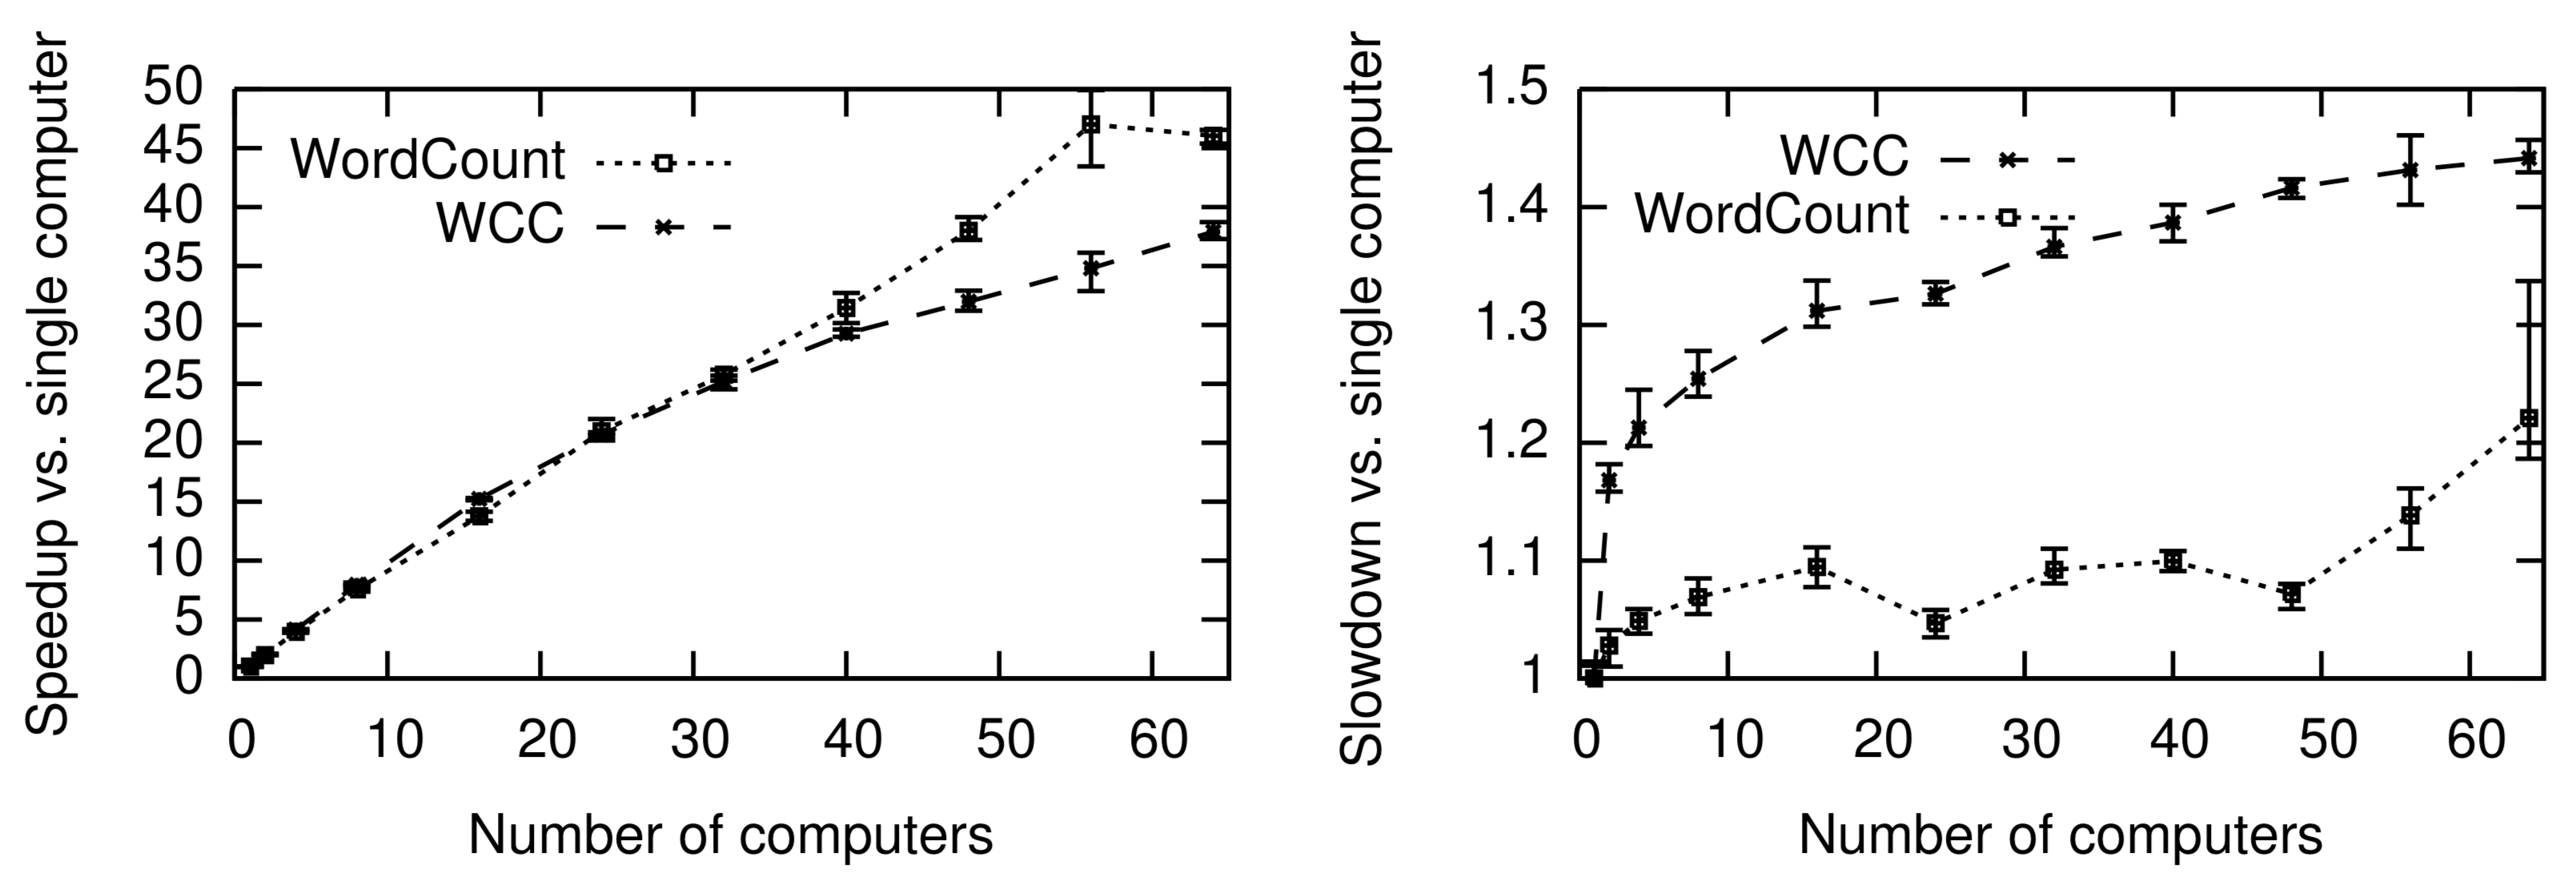
\includegraphics[width=1\textwidth]{6de}
  \end{center}
\end{frame}

\begin{frame}[t]{
  Real World Applications
  \only<2->{ - \\ ~Batch Iterative Graph Computation}
}
  \vspace{0.15cm}

  \only<2->{
    \begin{itemize}
      \setlength\itemsep{0.15cm}
      \item Graph Computation on Large scale real world datasets.
      \item PDW -- Distributed Database
      \item DryadLINQ -- General Purpose Batch Processor
      \item SHS -- Purpose Built Distributed Graph Store
      \item Speedups demonstrate the power of being able to maintain application-specific state in memory between iterations.
    \end{itemize}

    \vspace{0.15cm}
    \begin{center}
      \begin{figure}
        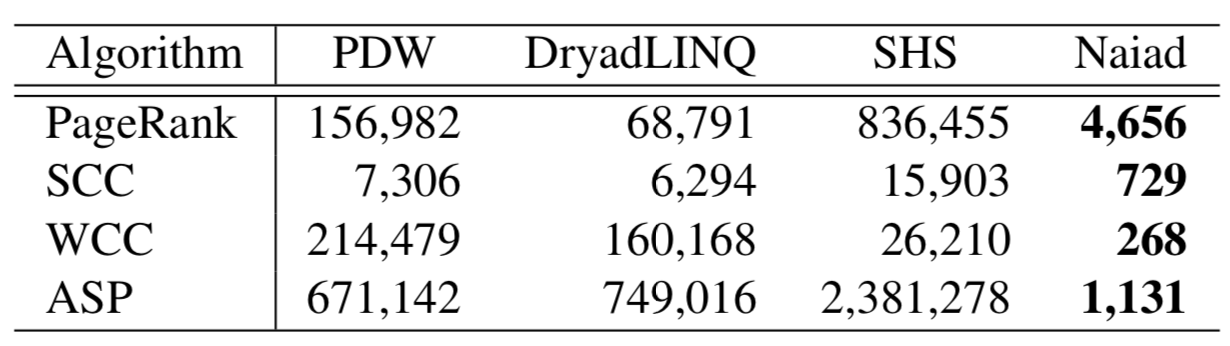
\includegraphics[width=0.85\textwidth]{t1}\\
        \small{Running time in seconds}
      \end{figure}
    \end{center}
  }
\end{frame}

\begin{frame}[t]{Batch Iterative Graph Computation}
  \vspace{0.15cm}

  \begin{itemize}
    \setlength\itemsep{0.15cm}
    \item Several systems have adopted the computation of PageRank on a Twitter follower graph as a standard benchmark.
    \item Naiad Vertex -- Partitions edges by source vertex.
    \item Naiad Edge -- Partitions edges using a space-filling curve. 
  \end{itemize}

  \vspace{0.15cm}
  \begin{center}
    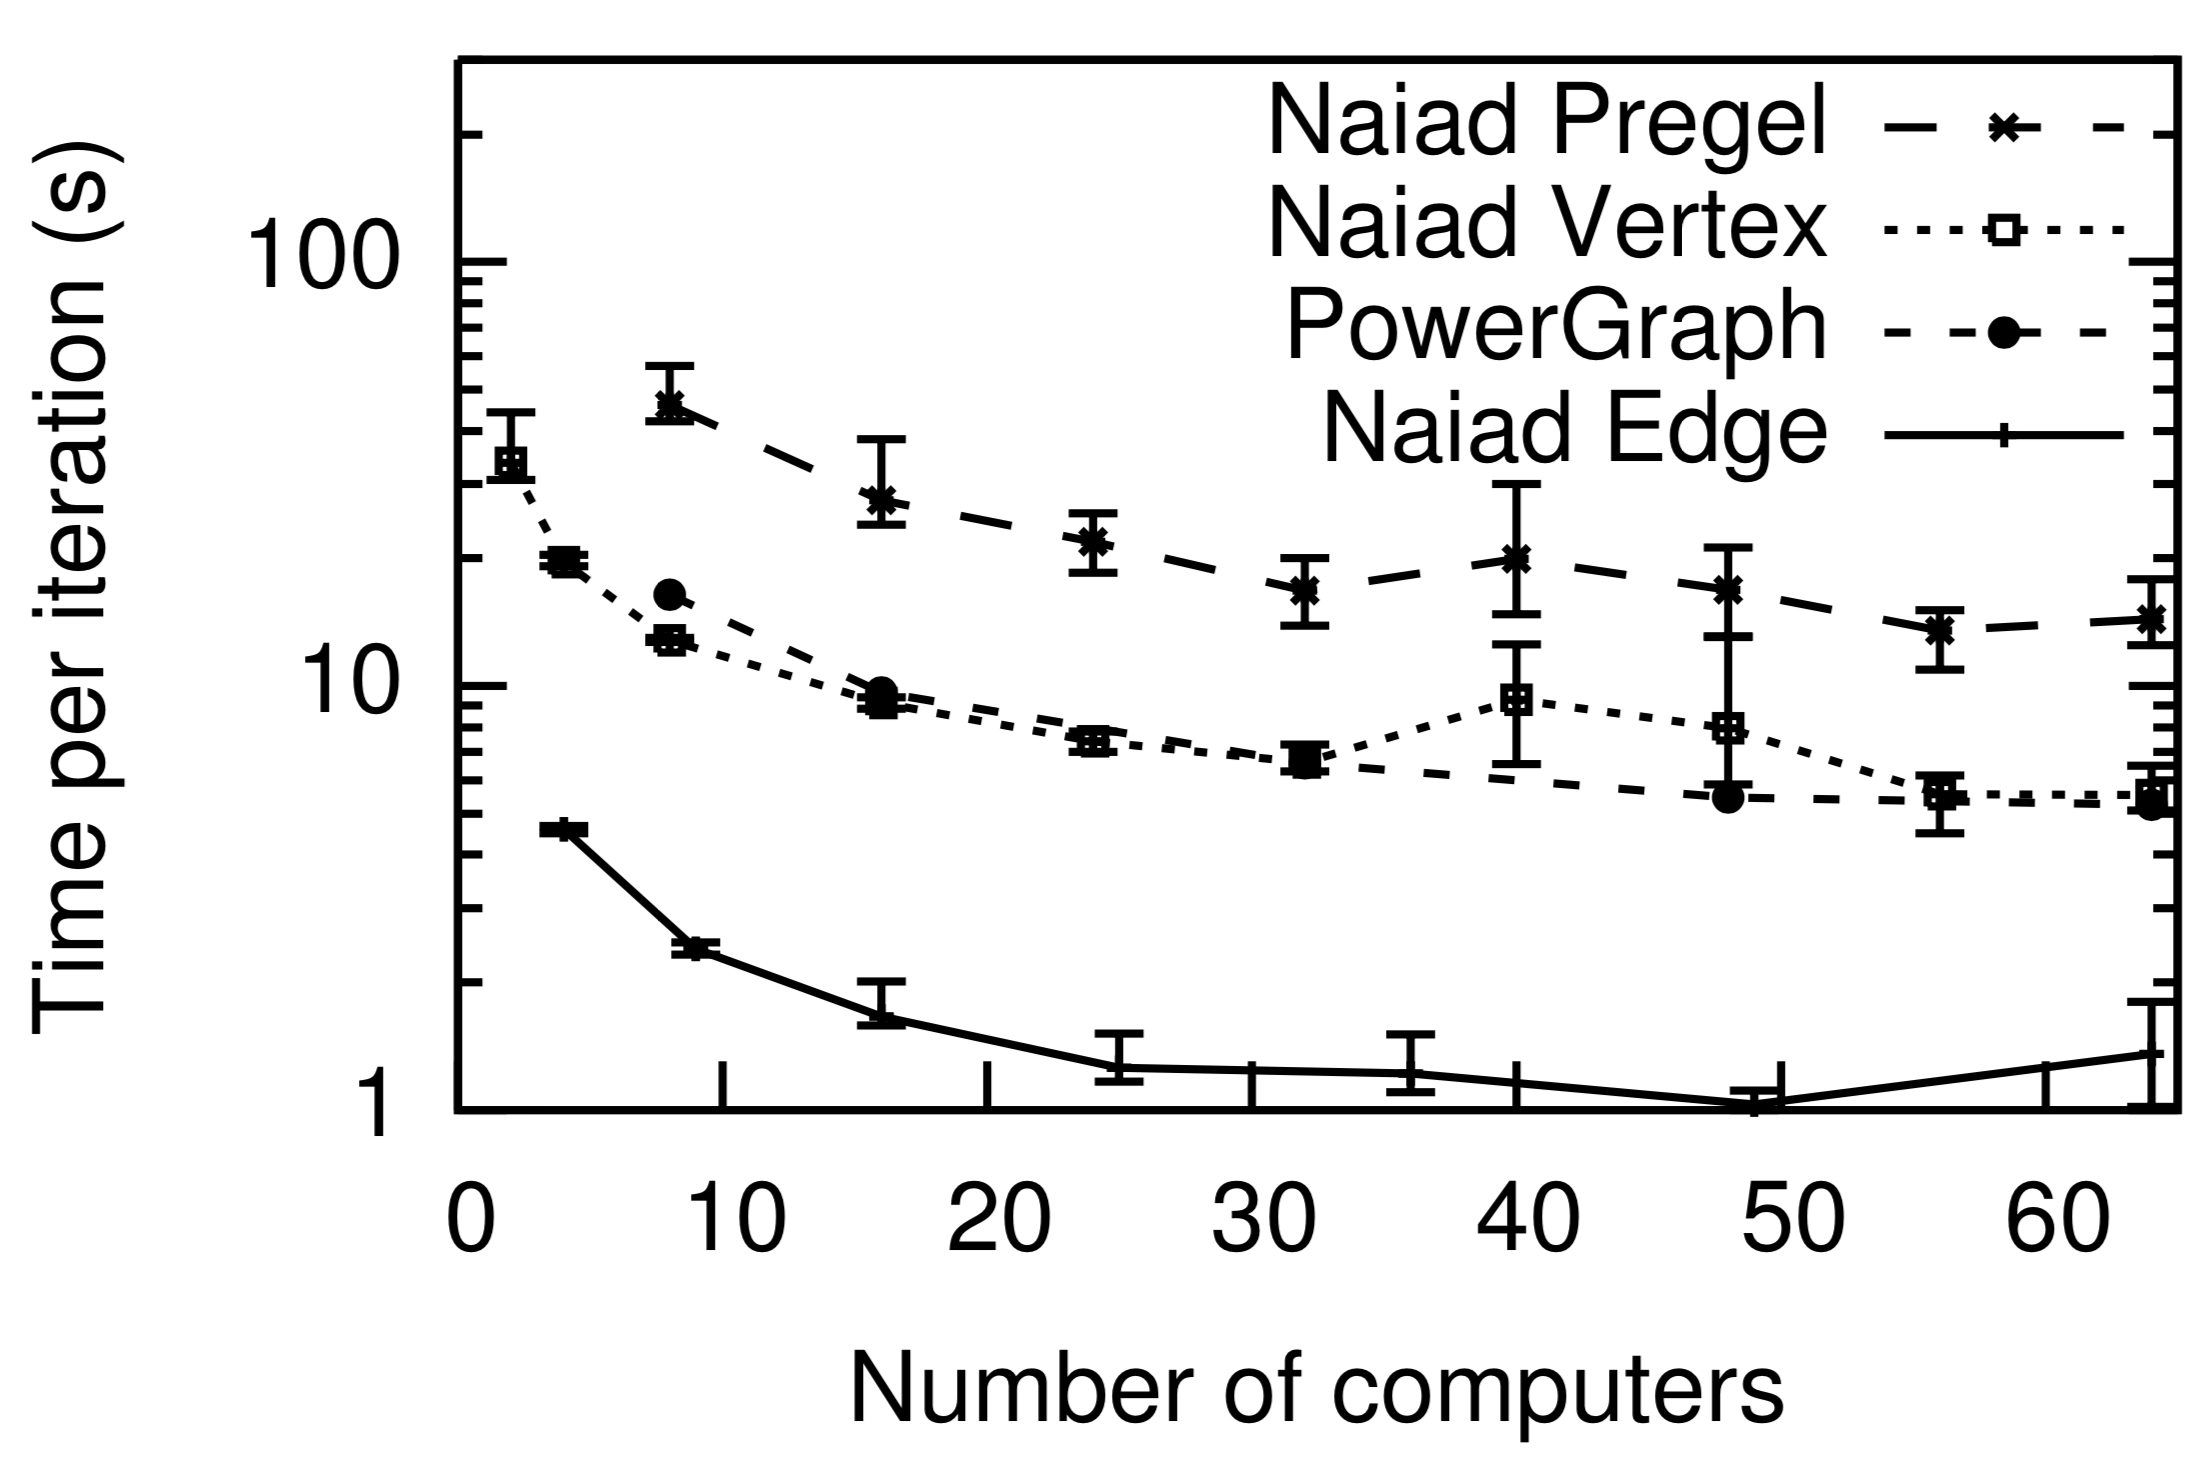
\includegraphics[width=0.55\textwidth]{7a}
  \end{center}
\end{frame}

\begin{frame}[t]{Batch Iterative Machine Learning}
  \vspace{0.15cm}

  \begin{itemize}
    \setlength\itemsep{0.15cm}
    \item Vowpal Wabbit (VW) -- open-source distributed machine learning library
    \item Modified VW -- \\first and second phases run inside a Naiad vertex, \\third phase uses Naiad implementation of the AllReduce.
  \end{itemize}

  \vspace{0.15cm}
  \begin{center}
    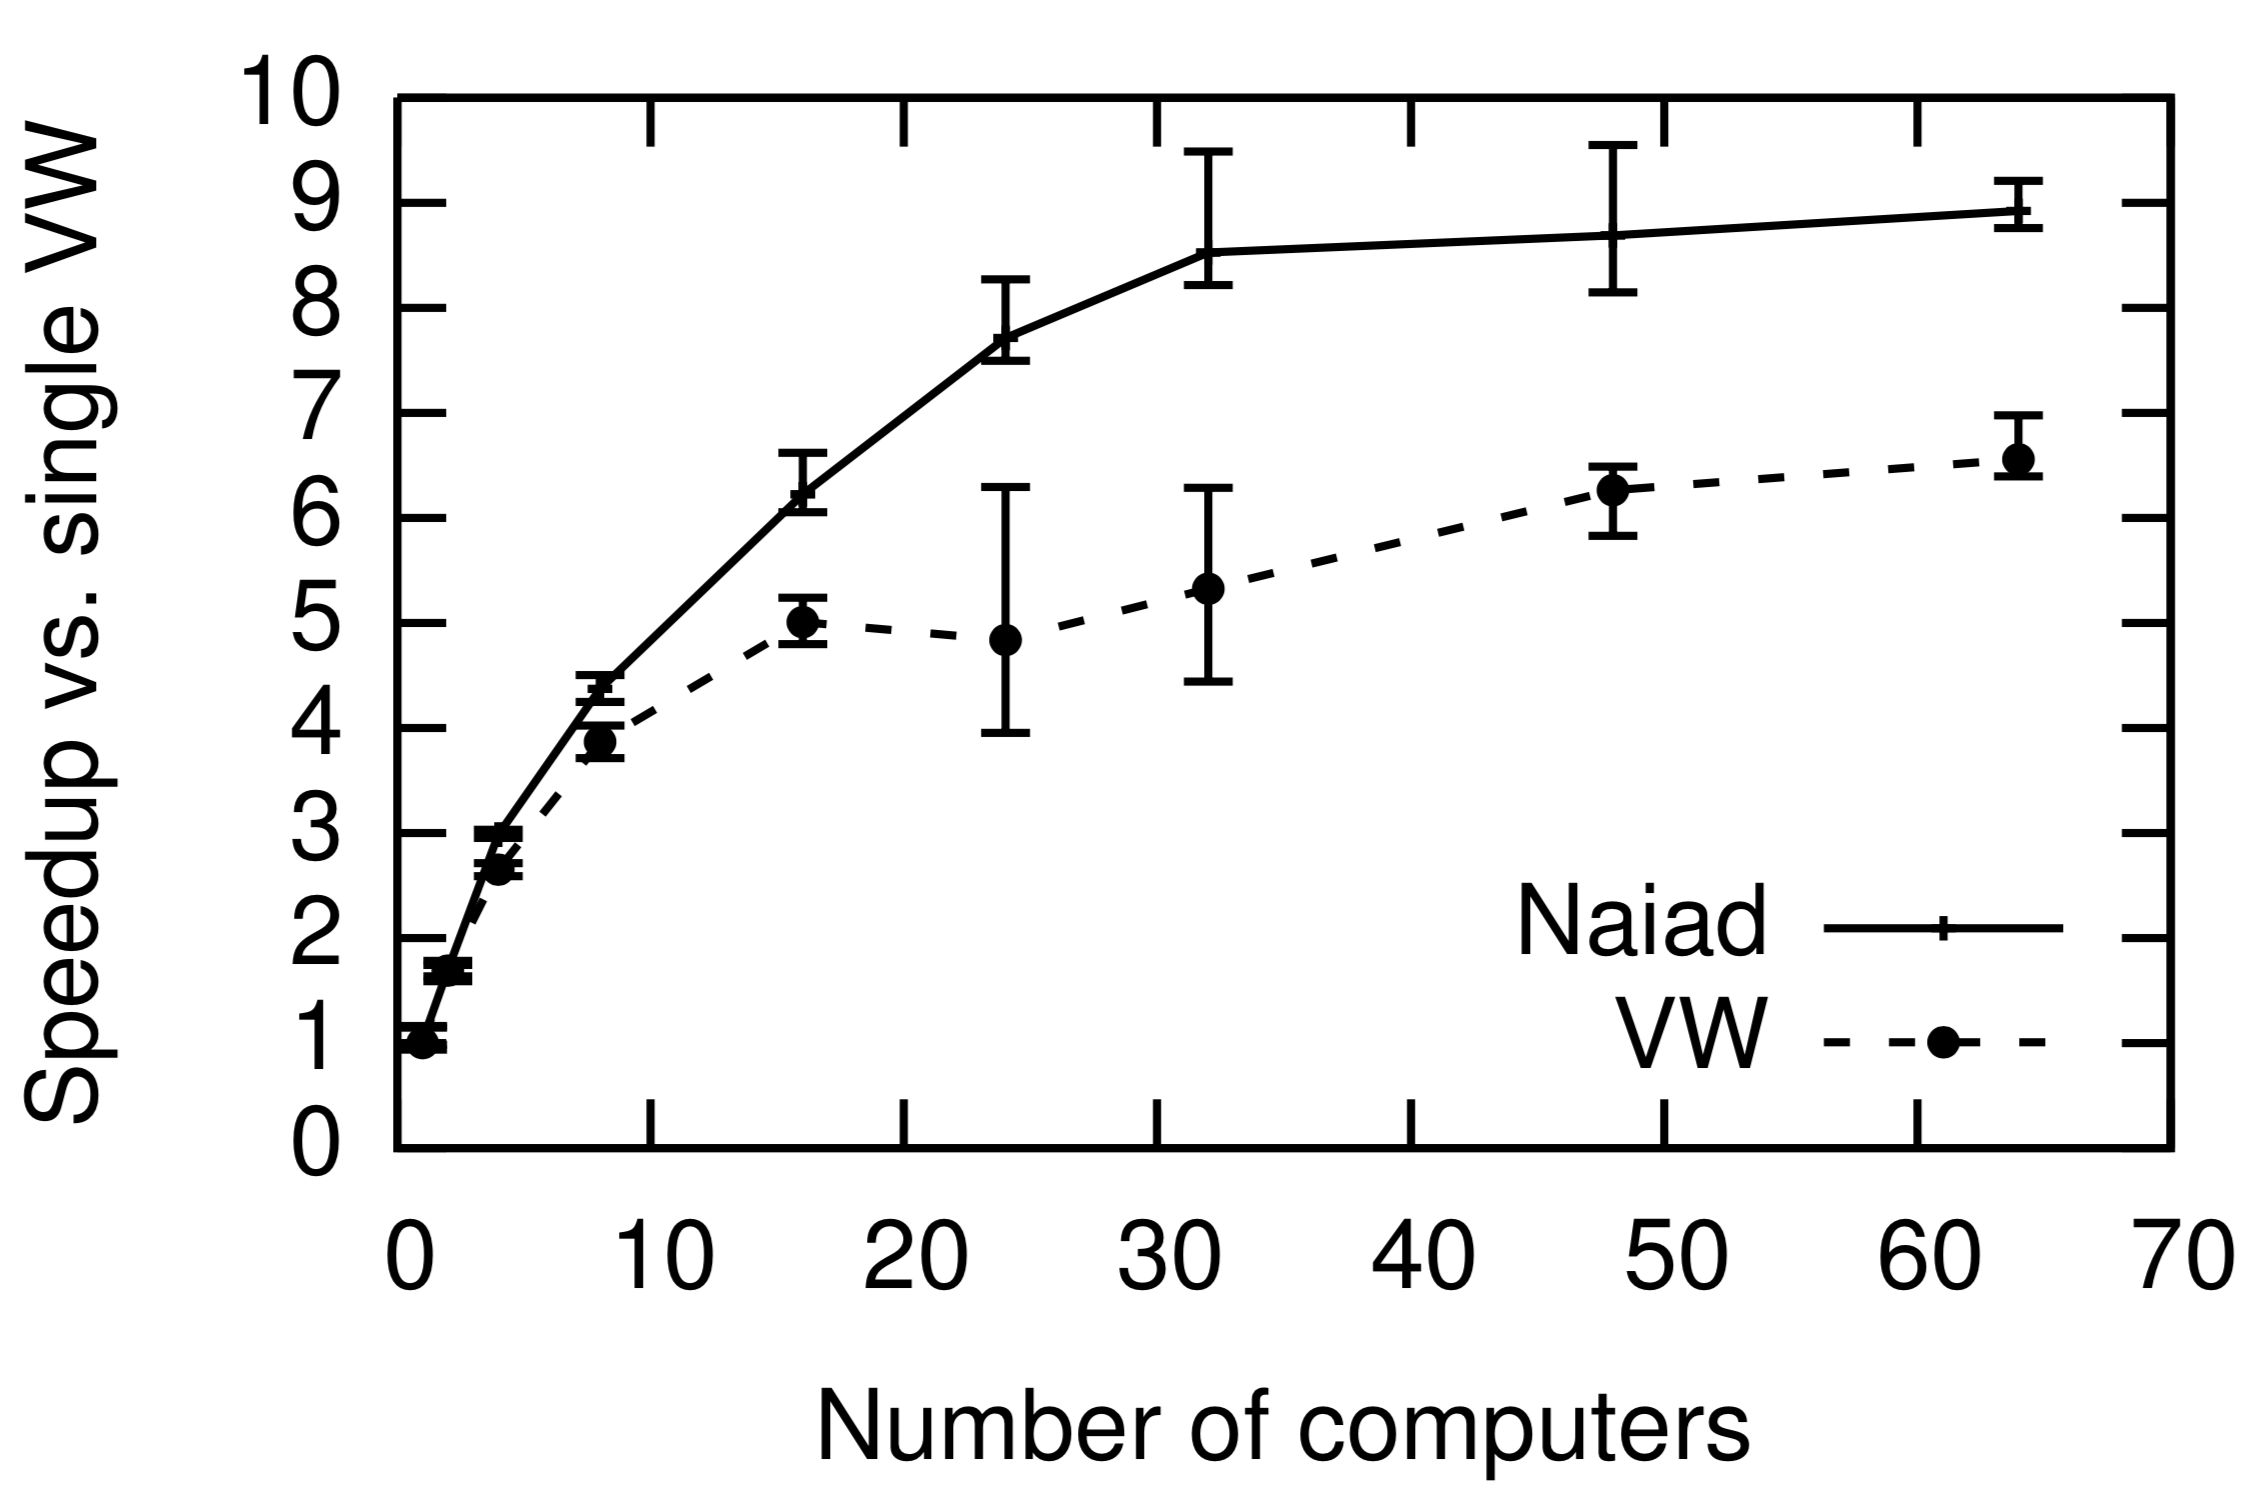
\includegraphics[width=0.55\textwidth]{7b}
  \end{center}
\end{frame}

\begin{frame}[t]{Streaming Acyclic Computation}
  \vspace{0.15cm}

  \begin{itemize}
    \setlength\itemsep{0.15cm}
    \item Kineograph ingests arriving graph data, takes regular snapshots for data parallel computation, and produces consistent results.
    \item The system is partitioned into ingest nodes and compute nodes.
    \item k-exposure metric for identifying controversial topics on Twitter.
  \end{itemize}

  \begin{center}
    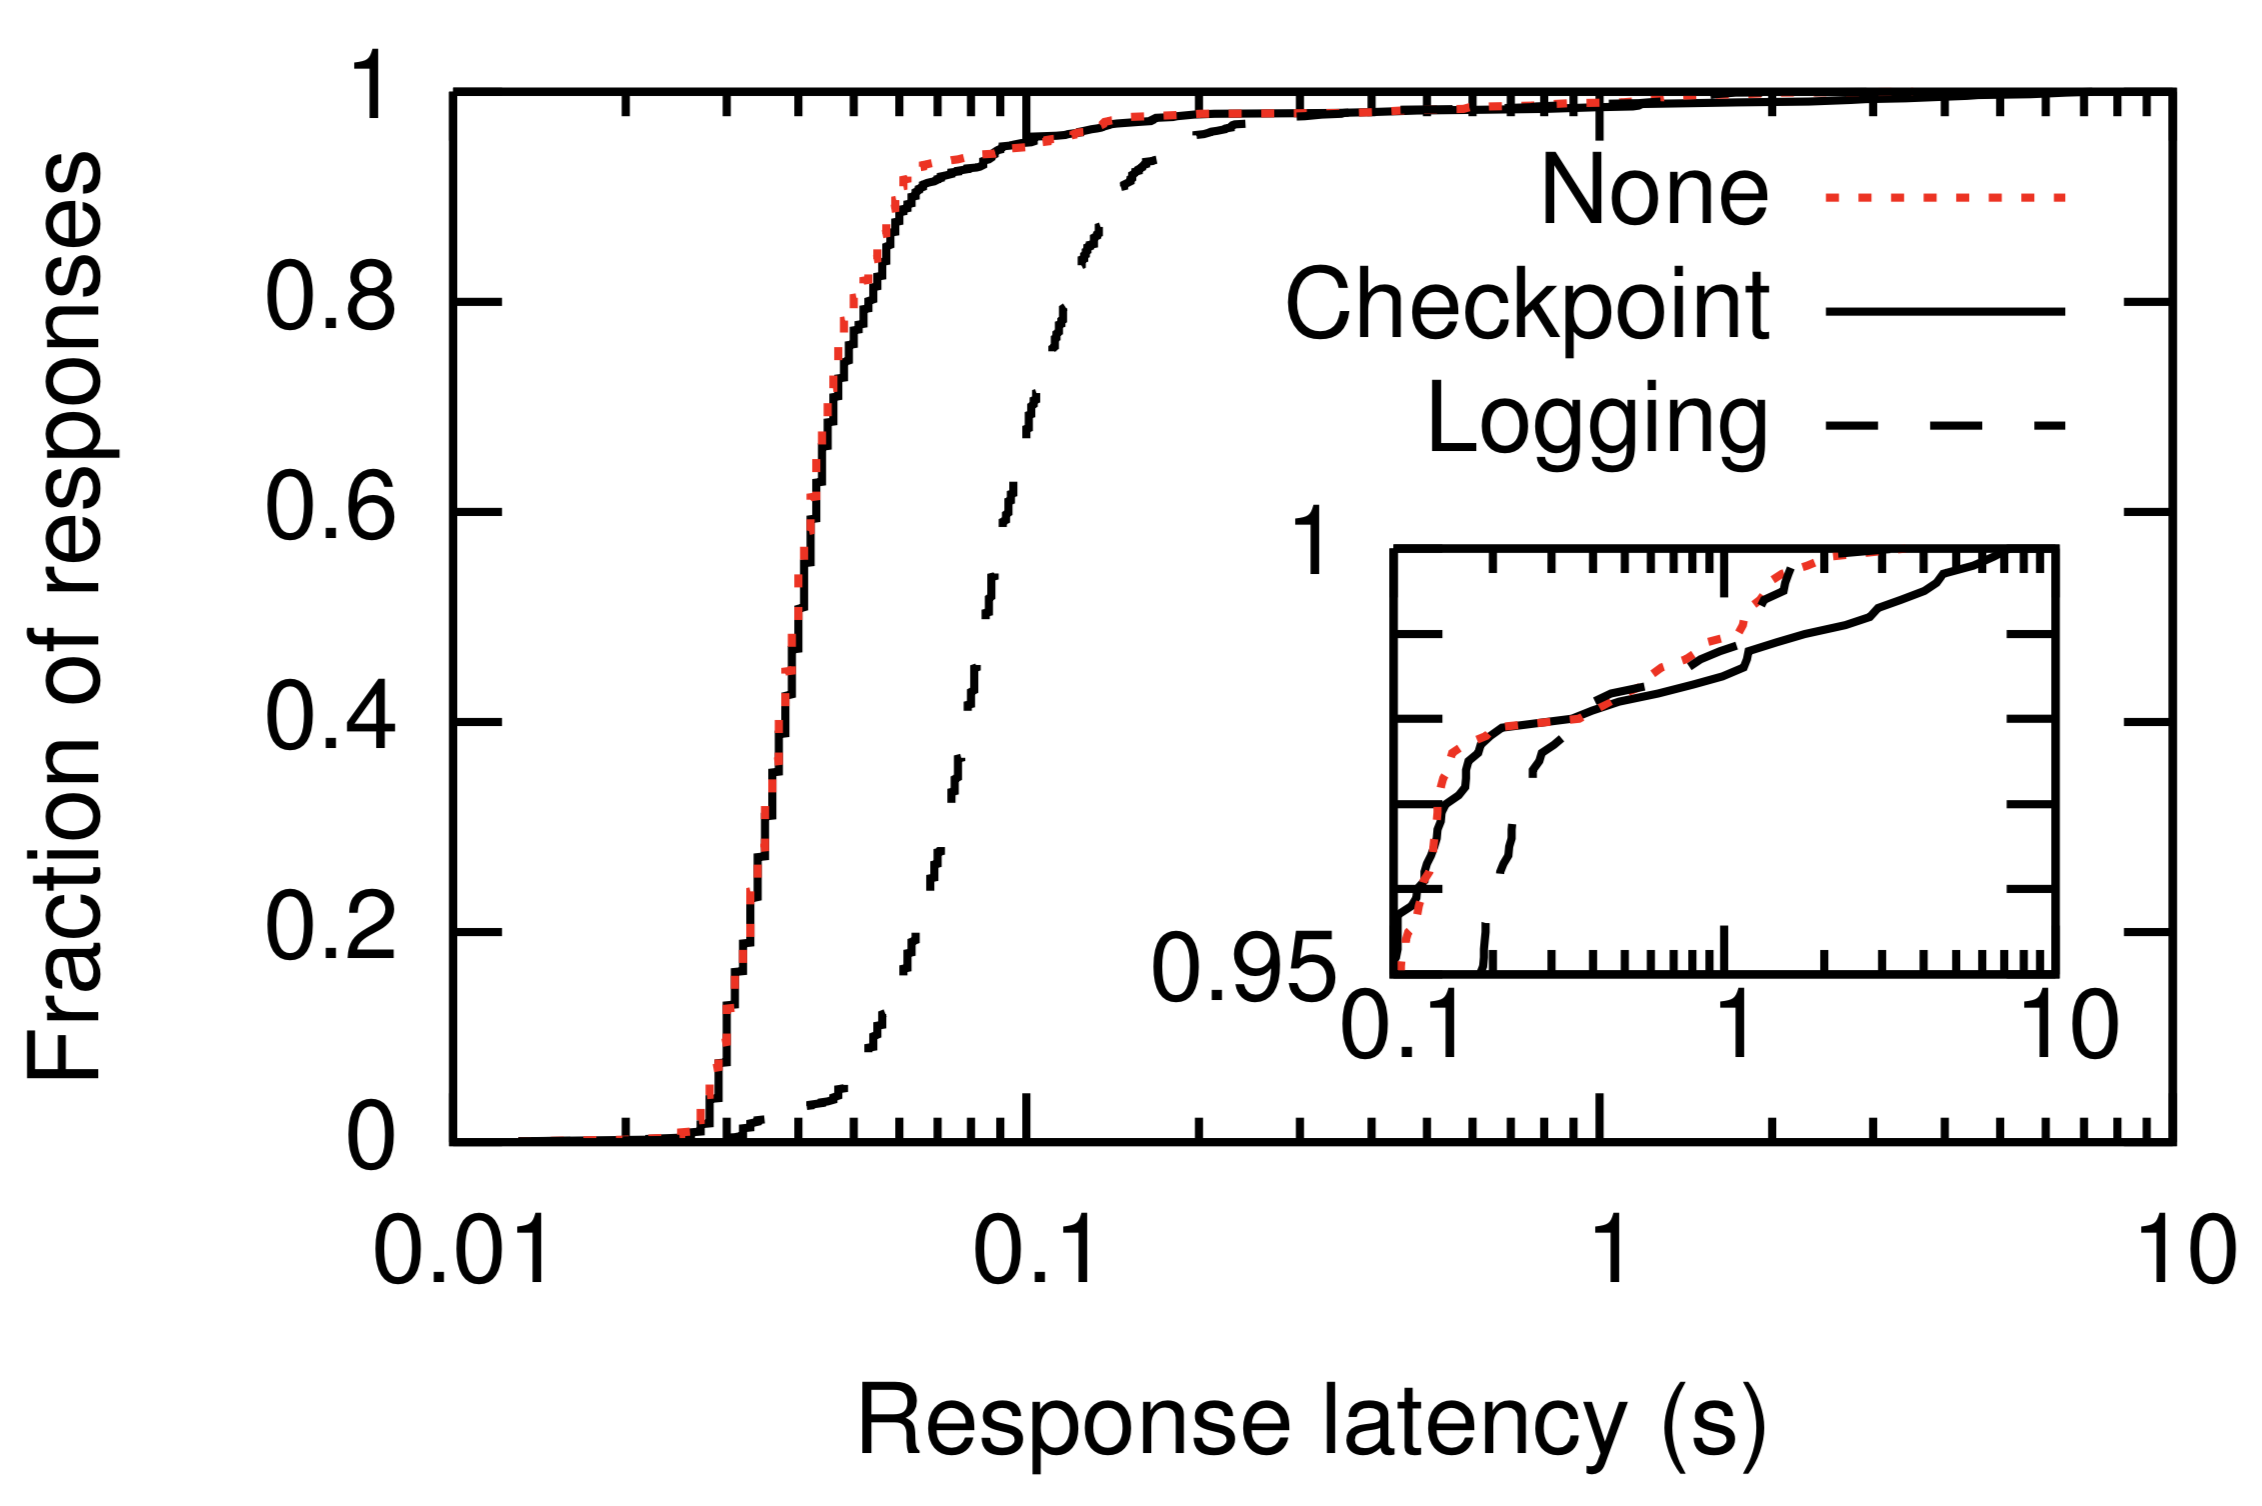
\includegraphics[width=0.55\textwidth]{7c}
  \end{center}
\end{frame}

\begin{frame}[t]{Streaming Iterative Graph Analytics}
  \vspace{0.15cm}

  \begin{itemize}
    \setlength\itemsep{0.15cm}
    \item There are two input stages: stream of tweets and requests, specified by a user name and query identifier.
    \item "Fresh" -- queries being delayed behind tweet processing
    \item "1s delay" -- the benefit of querying stale but consistent data.
    \item Naiad’s support for overlapped computation by trading off responsiveness for staleness.
  \end{itemize}

  \vspace{0.15cm}
  \begin{center}
    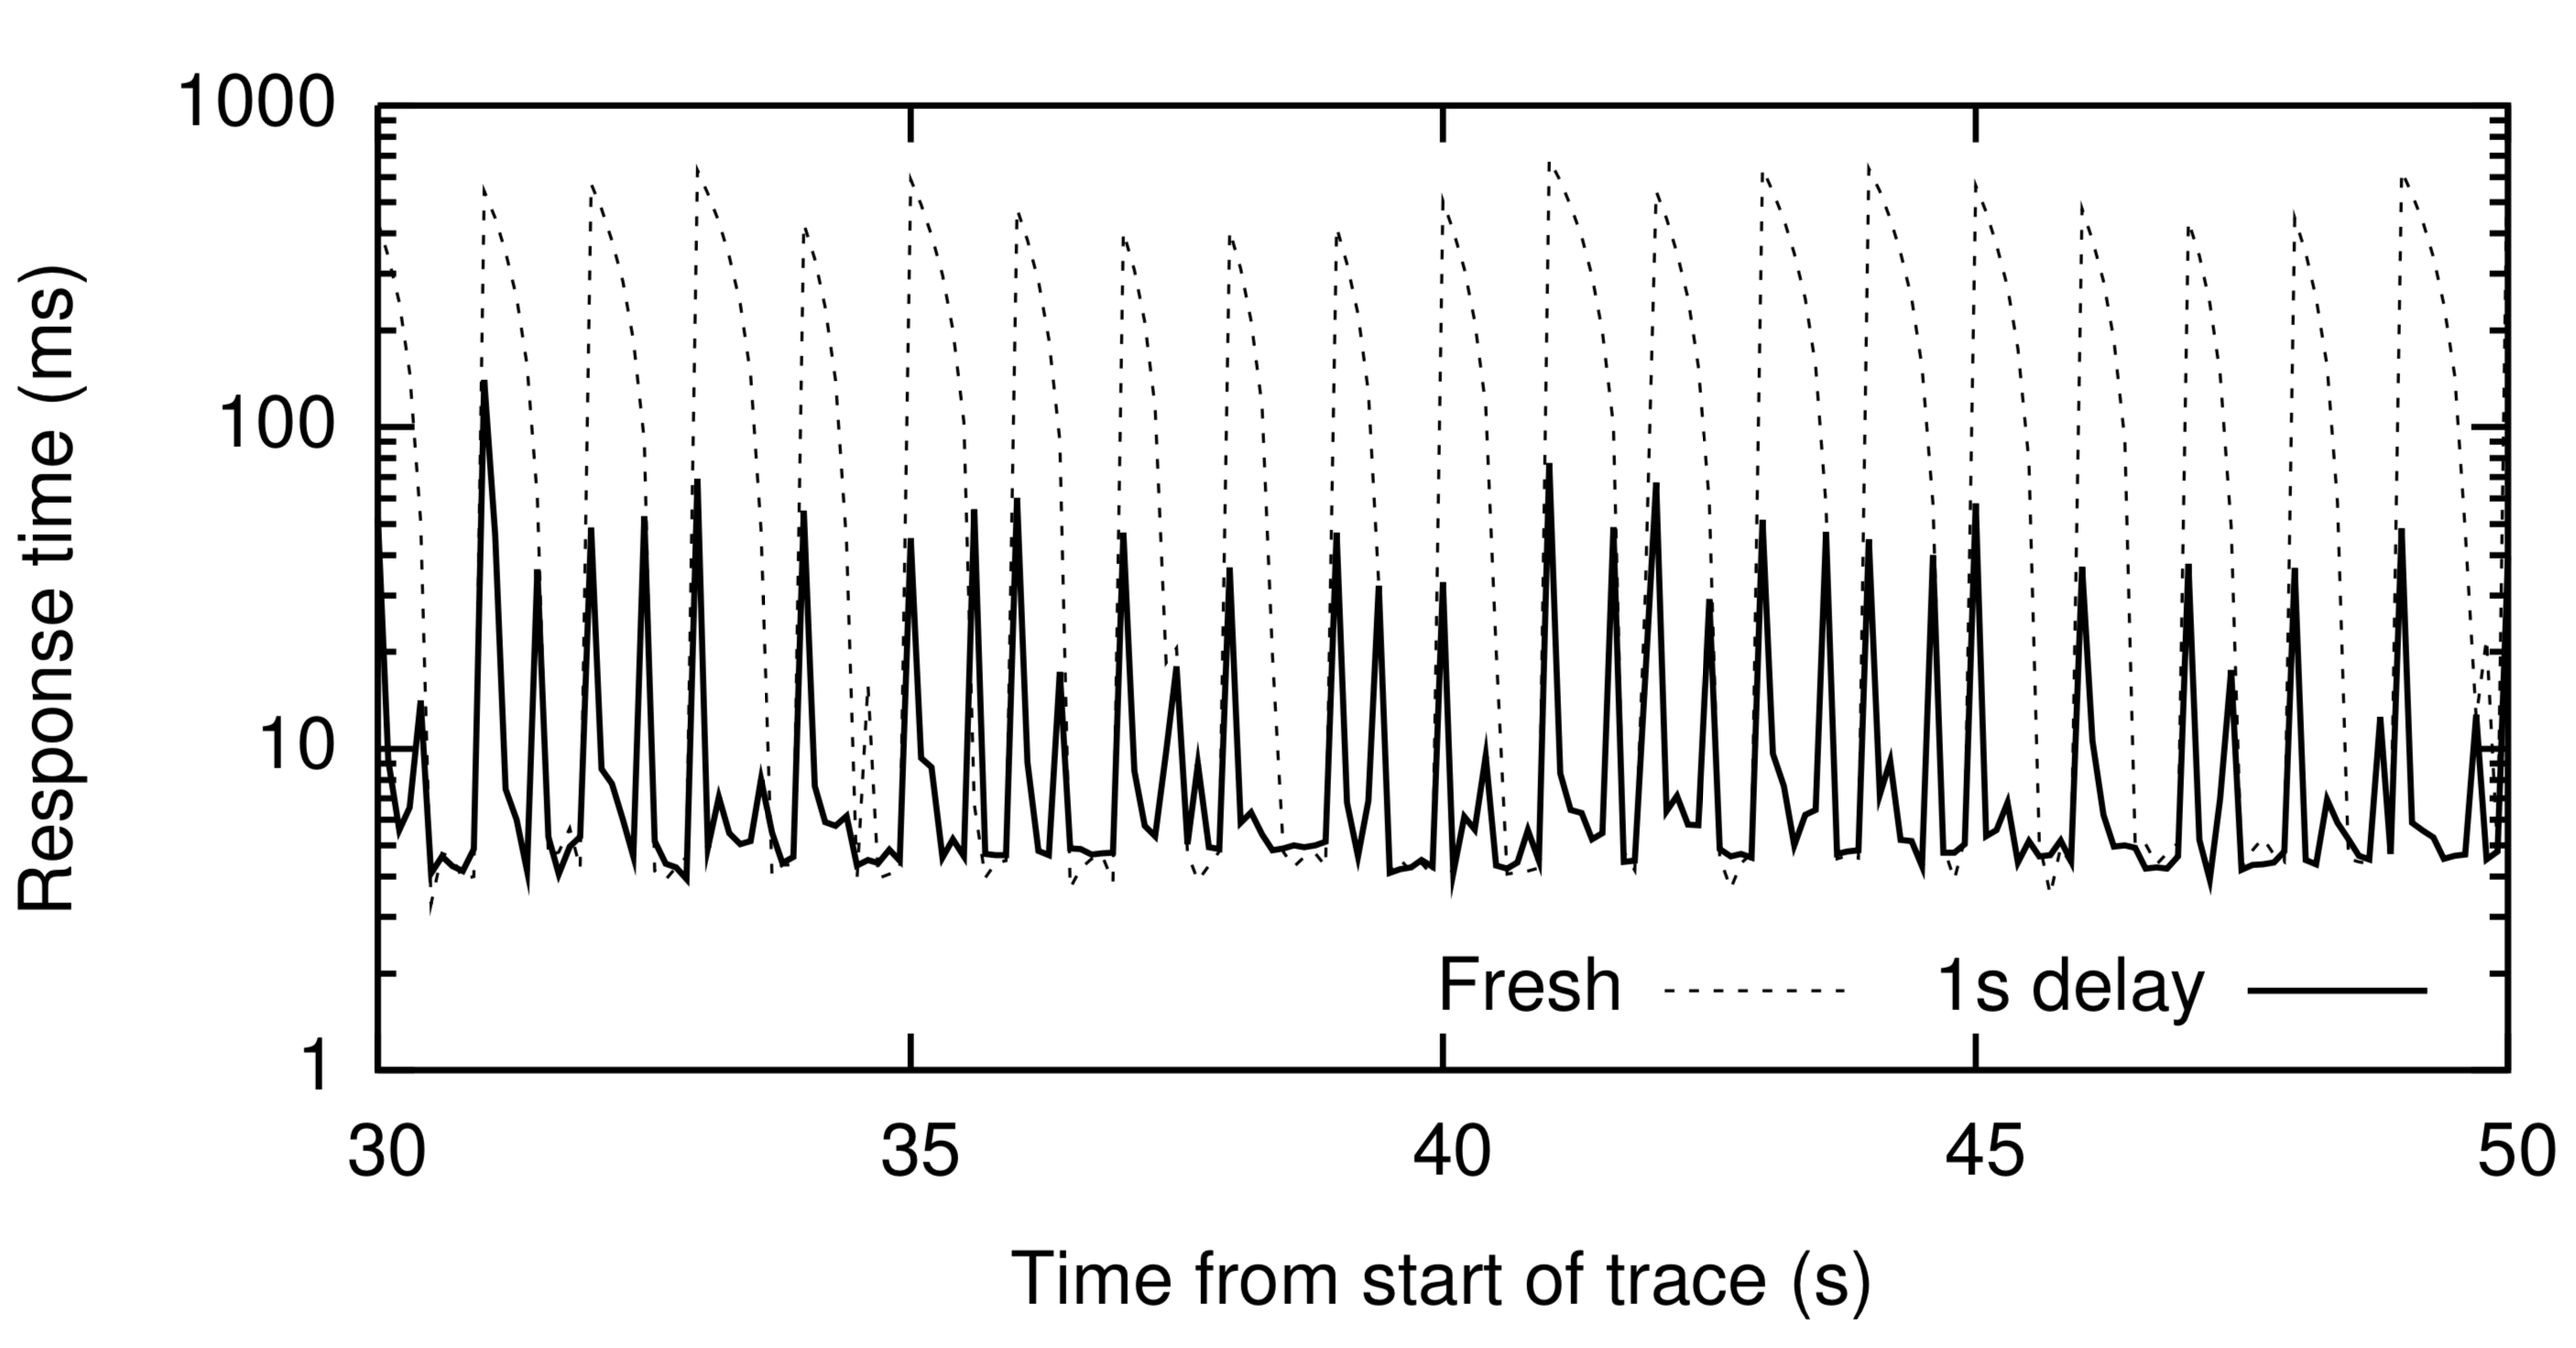
\includegraphics[width=0.70\textwidth]{8}
  \end{center}
\end{frame}